\documentclass{article}

\usepackage{../../austin137}
\usepackage{../../local}
\usehyperstuff

\usepackage{wrapfig}

\begin{document}

%%%%%%%%%%%%%%%%%%%%%%%%%%%%%%%%%%%%%%%%%%%%%%%%%%%%%%%%%%%%%%%%%%%%%%%%%%%%%%%%
\addcopyright
\begin{center}
{\bf \large Physics W89 - Introduction to Mathematical Physics - Summer 2023}\\\medskip
{\bf \large Problem Set - Module 10 - I'm Partial to This Module} \\\medskip
{\emph{Last Update: \today}}
\end{center}


\dphline\bigskip
%%%%%%%%%%%%%%%%%%%%%%%%%%%%%%%%%%%%%%%%%%%%%%%%%%%%%%%%%%%%%%%%%%%%%%%%%%%%%%%%
\section*{Problem 10.1 - A Convoluted Diffusion Problem\footnote{Return of the Puns!}}
\relevid{Some Important Linear PDEs in Physics;
Boundary Conditions;
Solving PDEs with the Fourier Transform;
Green's Functions}

%%%%%%%%%%%%%%%%%%%%%
\paragraph{}
Consider a diffusion problem in one dimension,
	\begin{equation*}
		\pdiff{\rho}{t} = \alpha\ppdiff{\rho}{x},
	\end{equation*}
where $\alpha>0$ is some diffusion constant and $\rho$ is some concentration of a substance in a long thin tube or fiber.  For example, maybe we've added some food
dye to a long thin pipe of still water.  If the distribution $\rho$ isn't uniform to start
it will diffuse/flatten out in a way specified by the diffusion equation.  Let $\rho(x,t)$ be the concentration of food dye at position $x$ in the tube at time $t$ and let
$R(k,t)$ be the Fourier transform from the space to the wave-number domain.

%%%%%%%%%%%%%%%%%%%%%
\paragraph{(a)}
In terms of $R(k,t)$ and its time derivatives, find the Fourier transforms of the derivatives that occur the diffusion equation. 
Use this to rewrite the diffusion equation as a system of decoupled 
\emph{ordinary} differential equations for $R(k,t)$ in the independent variable $t$.\\
\note{Your answer may not look like a system of ODEs but it is - there is one ODE for each possible $k$.}

\begin{solution}
	We remember that the derivative of the Fourier series just shifts the constants over by a factor 
	of $ik$ every time, therefore we get the following differential equation:
	\[
		\pdv{R(k, t)}{t} = \alpha (ik)^2 R(k, t) = -\alpha k^2 R(k, t)
	\] 
	As the note says, this is indeed a decoupled differential equation, one for each $k$. 
\end{solution}

%%%%%%%%%%%%%%%%%%%%%
\paragraph{(b)}
Solve your ODE from part (a) to find $R(k,t)$ given an initial concentration $R(k,0) \equiv R_{0}(k)$.
\spoilers{At the end of the day you should wind up with $R(k,t) = e^{-\alpha k^{2}t}R_{0}(k)$.}

\begin{solution}
	This is a linear, first order ODE in time. As we've seen in module 8, the solution to this ODE is of 
	the form:
	\[
		R(k, t) = A(k)e^{- \alpha k^2 t}
	\] 
	The constant $A(k)$ is the function that must be determined via an initial condition. We're given an 
	initial concentration of $R(k, 0) \equiv R_0(k)$, so therefore we plug in $t=0$:
	\[
	R(k, 0) = R_0(k) =  A(k)(1) \implies A(k) = R_0(k)
	\] 
	Therefore, our full solution is
	\[
		R(k, t) = R_0(k) e^{-\alpha k^2 t}
	\] 
\end{solution}
\phline
%%%%%%%%%%%%%%%%%%%%%
\paragraph{}
Suppose we start out with a Gaussian temperature distribution of width $\sigma$ at time $t=0$,
	\begin{equation*}
		\rho_{0}(x) = \frac{1}{\sqrt{2\pi\sigma^{2}}}e^{-x^{2}/2\sigma^{2}}.
	\end{equation*}
From Problem 9.5(d) we know the Fourier transform at time $t=0$ is
	\begin{equation*}
		R_{0}(k) = e^{-\sigma^{2}k^{2}/2}.
	\end{equation*}

%%%%%%%%%%%%%%%%%%%%%
\paragraph{(c)}
Use your result from (b) to find $\rho(x,t)$, the distribution of food dye as a function of time.
\spoilers{Your answer should still be a Gaussian.  You may want to define some constants to help simplify the algebra.}

\begin{solution}
	To find $\rho(x, t)$, we have to take the inverse Fourier transform of $R(k, t)$. We can do 
	this by applying the IFT formula:
	\begin{align*}
		\rho(x, t) &= \mathcal F^{-1}[R(k, t)](x, t)\\
				   &= \frac{1}{2\pi}\iinf e^{-\alpha k^2 t - \sigma^2 k^2 /2 + ikx} dk \\
				   &= \frac{1}{2\pi}\iinf e^{-(k^2(\alpha t + \sigma^2 /2) - (ix)k)} dk 
	\end{align*} 
	And now we remember this convenient formula from module 9:
	\[
		\iinf e^{-(ax^2 + bx)} dx = \sqrt{\frac{\pi}{a}} e^{b^2 / 4a}
	\] 
	For our integral, we have $a = \alpha t + \frac{\sigma^2}{2}$ and $b = -ix$, so therefore 
	this integral evaluates to:
	\[
		\rho(x, t) = \frac{1}{2\pi}\sqrt{\frac{\pi}{\alpha t + \frac{\sigma^2}{2}}} e^{(-ix)^2 / 4(\alpha t + \frac{\sigma^2}{2})}
	\] 
	After a bit of simplification (specifically, simplifying the square root), we get:
	\[
		\rho(x, t) = \frac{1}{\sqrt{2\pi(2\alpha t + \sigma^2)} }e^{-x^2 /4(\alpha t + \sigma^2 /2)}
	\] 
\end{solution}
%%%%%%%%%%%%%%%%%%%%%
\paragraph{(d)}
Find and graph the width of the Gaussian distribution as a function of time.
\extrasubpart{Make an animation of the diffusion!}

\begin{solution}
	The width is given by the standard deviation of the Gaussian. Comparing this to the formula for a 
	standard Gaussian:
	\[
		f(x) = \frac{1}{\sqrt{ 2\pi \sigma'^2}}e^{-x^2 / 2 \sigma'^2}
	\] 
	We can see that the width is given by the factor next to $\sqrt{2\pi}$ in the prefactor. Here, 
	I'm using primes to not confuse with $\sigma$ in $\rho(x, t)$. Therefore, based on this logic of comparing,
	we see that
	\[
	\sigma'^2 = 2\alpha t + \sigma^2 \implies \sigma'(t) = w(t) = \sqrt{2\alpha t + \sigma^2} 
	\] 
	As for the graph, here it is, with $\sigma = 1$ and $t = 1$, for simplicity:
	\begin{center}
		\begin{tikzpicture}[domain=0:8, samples=300]
			\draw[thick](-1, 0) -- (10, 0) node[right] {$t$};
			\draw[thick](0, -2) -- (0, 2) node[above] {$w$};
			\draw[color=blue] plot (\x, {(2* \x + 1)^(1/2)}) node[right]
				{$w(t) = \sqrt{2\alpha t + \sigma^2} $};
		\end{tikzpicture}
	\end{center}
	Physically speaking, this also makes sense, since the temperature will try to even itself out across
	the entire length of the tube, until the entire tube is of constant temperature, at which point the 
	width of our Gaussian is effectively infinite. This is exactly what the limit of our graph and function 
	suggests as well, so it's a good sanity check.
\end{solution}

\phline
%%%%%%%%%%%%%%%%%%%%%
\paragraph{}
Your Fourier transform from part (b) is a product of two functions of $k$ and thus two Fourier transforms.  
We already have that $R_{0}(k)$ is the Fourier transform of our initial condition $\rho_{0}(x)$.
Define $H(k,t) = e^{-\alpha k^{2}t}$ so that $R(k,t) = H(k,t)c_{0}(k)$ and let $h(x,t)$ be the inverse Fourier transform of $H(k,t)$.  

%%%%%%%%%%%%%%%%%%%%%
\paragraph{(e)}
Find $h(x,t)$, the inverse Fourier transform of $H(k,t)$.  Then write $\rho(x,t)$ as a convolution integral involving $h(x,t)$.  Finally, solve for 
$\rho(x,t)$ given a point source initial condition $\rho_{0}(x) = \delta(x-x_{0})$.\\
\note{Your answer will be the (position) \heavydef{Green's function} for diffusion in 1D, $G(x,x_{0},t)$}

\begin{solution}
	We begin by taking the inverse Fourier transform using the formula:
	\[
		f(x) = \frac{1}{2\pi}\iinf c(k) e^{ikx} dk 
	\] 
	Therefore, we can find $h(x, t)$:
	\begin{align*}
		h(x, t) &= \frac{1}{2\pi}\iinf H(k, t) e^{ikx} dk \\
				&= \frac{1}{2\pi}\iinf e^{-\alpha k^2 t} e^{ikx} dk \\
				&= \frac{1}{2\pi}\iinf e^{-(\alpha k^2 t - (ix)k)} dk 
	\end{align*}
	We use the same integral trick as we did in part (c), which gives us:
	\begin{align*}
		h(x, t) &= \frac{1}{2\pi}\sqrt{\frac{\pi}{\alpha t}} e^{-x^2 / 4 \alpha t}\\
				&= \frac{1}{2\sqrt{\pi \alpha t} }e^{-x^2 / 4\alpha t}
	\end{align*}
	Now, to write $\rho(x, t)$ as a convolution, we first recognize that $\rho(x, t)$ can be obtained 
	as the inverse Fourier transform of $R(k, t) = H(k, t) c_0(k)$. Since $R(k, t)$ is a product of two 
	functions, we can use the convolution theorem here:
	\[
		\rho(x, t) = \mathcal F^{-1}[R(k, t)](x, t) = \mathcal F^{-1}[H(k, t)c_0(k)] = (h \ast \rho_0)
		(x, t)
	\] 
	And now we can write out the convolution, and also using the fact that $\rho_0(x) = \delta(x - x_0)$:
	\[
		\rho(x, t) = \iinf h(x - s, t) \delta(s - x_0) ds
	\]
	And now we can use the property of the dirac delta:
	\[
	\int_a^b f(x) \delta(x - x_0) = \begin{cases}
		f(x_0) & a < x_0 < b\\ 
		0 &\text{else}
	\end{cases}
	\] 
	So this expression simplifies to:
	\[
	\rho(x, t) = \iinf h(x - s, t) \delta(s - x_0) ds = h(x - x_0, t) = \frac{1}{2\sqrt{\pi \alpha t} }
	e^{-(x - x_0)^2 / 4\alpha t}
	\] 
\end{solution}

\bigskip
\dphline
\pagebreak
%%%%%%%%%%%%%%%%%%%%%%%%%%%%%%%%%%%%%%%%%%%%%%%%%%%%%%%%%%%%%%%%%%%%%%%%%%%%%%%%
\section*{Problem 10.2 - Separation of Variables on a Square Drumhead}
\relevid{Separation of Variables - Motivation;
Solving PDEs with Separation of Variables;
Separation of Variables and Boundary Value Problems}

\paragraph{}
Consider a 2D wave equation for a square region $0\leq x \leq L$ and $0\leq y \leq L$,
	\begin{equation*}
		\ppdiff{u}{t} = v^{2}\nabla^{2}u = v^{2}\left(\ppdiff{u}{x}+\ppdiff{u}{y}\right).
	\end{equation*}

%%%%%%%%%%%%%%%%%%%%%
\paragraph{(a)}
Perform a separation of variables $u(x,y,t) = S(x,y)T(t)$ on the wave equation to get an ordinary differential equation for $T(t)$ and another
partial differential equation for $S(x,y)$.  In your separation of variables, you will need to introduce a separation constant for the time equation, a separation constant
for the space equation, and an algebraic relation between the two constants.

\begin{solution}
	We carry out the algebra for the separation of variables, exactly as it was done in lecture. Because the 
	functions are separated, $T(t)$ will not be affected by space derivatives, and $S(x, y)$ will not be 
	affected by time derivatives. Doing the algebra:
	\begin{align*}
		S(x, y) \pdv[2]{T}{t}(t) &= T(t) v^2 \nabla^2 S(x, y) \\
		\pdv[2]{T}{t}(t) \cdot \frac{1}{T} &=  \frac{v^2}{S(x, y)}\nabla^2 S(x, y) 
	\end{align*}
	Now moving everything to one side, we get:
	\[
		\frac{\ddot T}{T} - \frac{v^2}{S}\nabla^2 S = 0
	\] 
	Here, we see that the first function is purely a function of time, and the second is one of space. 
	Therefore, we have an equation of the form $f(t) - g(s) = 0$, meaning that both of these must be constants.
	Let $f(t) = c_t$ and $g(x, y) = c_{xy}$, then the equation gives us that $c_t - c_{xy} = 0$ so our algebraic 
	relation is $c_t = c_{xy}$. Now, if we write $c_t = c$, then we get the following set of differential
	equations:
	\begin{align*}
		\ddot T(t) &= cT(t)\\
		\nabla^2 S(x, y) &= \frac{c}{v^2}S(x, y)
	\end{align*}
\end{solution}
\phline
%%%%%%%%%%%%%%%%%%%%%
\paragraph{}
Suppose our system is a piece of elastic stretched over a square rim, like a drumhead.  The elastic is fixed to the rim, so we get the following
Dirichlet boundary conditions:
	\begin{enumerate}
		\item $u(0,y,t) = 0$\quad (Left side of rim fixed in place at height $u=0$.)
		\item $u(L,y,t) = 0$\quad (Right side of rim fixed in place at height $u=0$.)
		\item $u(x,0,t) = 0$\quad (Bottom side of rim fixed in place at height $u=0$.)
		\item $u(x,L,t) = 0$\quad (Top side of rim fixed in place at height $u=0$.)
	\end{enumerate}	
For the time evolution we will give initial conditions and see how the wave evolves.  This means specifying the initial configuration and velocities,
	\begin{enumerate}
		\setcounter{enumi}{4}
		\item $u(x,y,0) = u_{0}(x,y)$\quad (Fixed initial shape.)
		\item $\dot{u}(x,y,0) = v_{0}(x,y) = 0$\quad (Initial shape initially at rest.)
	\end{enumerate}

\paragraph{}
Suppose we have two separable solutions to the wave equation $u_{1}(x,y,t)$ and $u_{2}(x,y,t)$ that both satisfy all of the boundary conditions and initial conditions described
above. Let $u_{3}(x,y,t)$ be a linear combination $a\,u_{1}(x,y,t)+b\,u_{2}(x,y,t)$.  
Since the wave equation is linear, this will be a solution to the wave equation (though not necessarily a
separable one).


%%%%%%%%%%%%%%%%%%%%%
\paragraph{(b)}
Which of the above boundary and initial conditions will $u_{3}(x,y,t)$ be guaranteed to satisfy?  Translate the ``superposable'' boundary conditions and initial conditions
into conditions on the separated functions $T(t)$ and $S(x,y)$.\\
\note{There may be some specific $u_{0}(x,y)$, $a$, or $b$ that will allow the superposition to still satisfy all boundary conditions but these are special cases that we will
not consider here.}

\begin{solution}
	Writing $u_3(x, y, t) = a u_1(x, y, t) + bu_2(x, y, t)$, we see that the only initial conditions that 
	are guaranteed to be satisfied are when the initial condition doesn't depend on $a$ or $b$.\footnote{Equivalently, this is the same as identifying which Dirichlet and Neumann conditions 
	are set to zero, which are all the conditions except condition \#5.} In other 
	words, this means that the only initial conditions that are guaranteed to be satisfied are the 
	ones in which $u_i(x, y, t) = 0$ or $\dot u_i (x, y, t) = 0$. Therefore, all the initial conditions except
	the fifth one can be 
	satisfied automatically. As for the restrictions on $S$ and $T$:
	\begin{enumerate}[label=\alph*)]
		\item Condition 1: $u(0, y, t) = 0 \implies S(0, y) = 0$
		\item Condition 2: $u(L, y, t) = 0 \implies S(L, y) = 0$
		\item Condition 3: $u(x, 0, t) = 0 \implies S(x, 0) = 0$
		\item Condition 4: $u(x, L, t) = 0 \implies S(x, L) = 0$
		\item Condition 6: $\dot u(x, y, 0) = S(x, y) \dot T(0) = 0 \implies \dot T(0) = 0$
	\end{enumerate}
\end{solution}

\phline
%%%%%%%%%%%%%%%%%%%%%
\paragraph{}
Spoilers!  If you did things right in part (a), after you use the algebraic relation among the separation constants, your pair of DEs should be
	\begin{equation*}
		\ddot{T}(t) = -cT(t),	\qquad	\nabla^{2}S(x,y) = -\frac{c}{v^{2}}S(x,y).
	\end{equation*}
Define the constant $k\equiv \sqrt{c}/v$ so our separated equations become
	\begin{align}
		\frac{d^{2}T_{k}}{dt^{2}} &= -(kv)^{2}T_{k}(t),	\label{Tequation}\\	
		\nabla^{2}S_{k}(x,y) &= -k^{2}S_{k}(x,y).		\label{Sequation}
	\end{align}
I have included the separation constant $k$ as a subscript to the functions $T(t)$ and $S(x,y)$ to index which separable solution we are talking about.  Note that since we
haven't restricted $c$ to be positive or negative, $k$ may still be real or imaginary.

%%%%%%%%%%%%%%%%%%%%%
\paragraph{(c)}
Solve the time equation Eq.~\ref{Tequation} to get two linearly independent functions of time for a given $k$.  
Do this in two separate cases:  first when $k$ is real (for the case where $c>0$) and second when
$k=i\kappa$ is purely imaginary (for the case where $c<0$).  Impose the relevant boundary conditions on $T_{k}(t)$ from part (b).  Finally, use the fact
that we don't want our wave to blow up as $t\to\infty$ to argue that only the solutions with $k$ real are physically relevant.
\spoilers{When $k$ is real you should end up with the solution $\cos(kvt)$.  When $k$ is purely imaginary you should end up with the solution $\cosh(\kappa vt)$.}

\begin{solution}
	Let's start with the case where $k$ is real. We've seen this differential equation solved in lecture, 
	and its solution is:
	\[
		T_k(t) = Ae^{ikvt} + Be^{-ikvt}
	\] 
	Instead of these solutions though, I'll use the trigonometric ones instead:
	\[
	T_k(t) = A\cos(kvt) + B \sin(kvt)
	\] 
	This is because the initial conditions are much easier to plug into sine and cosine functions as opposed
	to complex exponentials. Either way though, they will lead to the same answer at the end of the day. 
	Now, let's start with the first boundary condition on $T$: $U(x, y, 0) = u(x, y)$, or in other words 
	$S(x, y) T(0) = S(x, y) \implies T(0) = 1$. Plugging this in:
	\[
	T_k(0) = 1 = A
	\] 
	So we find that $A = 1$. For the second initial condition, we have $\dot T(0) = 0$, therefore:
	\[
		\dot T_k(0) = B(kv) = 0 \implies B = 0
	\] 
	So therefore, we end up with a final solution of $T_k(t) = \cos(kvt)$, exactly as we should get
	according to the spoiler. When $k$ is complex (so $k = i\kappa$), we have the solution:
	\[
		T_k(t) = Ae^{i(i \kappa vt)} + Be^{-i(i \kappa vt)} = Ae^{-\kappa vt} + Be^{\kappa vt}
	\] 
	Again, plugging in the first boundary condition:
	\[
	T_k(0) = A + B = 1 
	\] 
	This gets us the first of two equations. Now we plug in the second initial condition:
	\[
	\dot T(0) = 0 \implies -\kappa vA + \kappa vB = 0
	\] 
	So we get $-A + B = 0$, or equivalently $A = B$. Combining this relation with the earlier one that $A + B 
	= 1$, we get that $A = B = \frac{1}{2}$. Therefore, our solution is of the form:
	\[
		T_k(t) = \frac{1}{2}\left( e^{-\kappa vt} + e^{\kappa vt} \right) 
	\] 
	Now we can head over to google and find that this is exactly the expression for the hyperbolic cosine:
	\[
		\cosh(kx) =\frac{1}{2}\left( e^{-kx} + e^{kx} \right) 
	\] 
	So for us, this means that our solution $T_k(t) = \cosh(kvt)$, again as we should get according to the 
	spoiler. Now for the final part of the problem: notice that when $k$ is imaginary, then depending on 
	the sign of $v$, one of the exponentials $e^{\kappa vt}$ or $e^{-\kappa vt}$ will grow exponentially.
	Specifically, 
	when $v > 0$, then $e^{\kappa vt}$ blows up as $t$ goes to infinity, and when $v < 0$, then 
	$e^{-\kappa vt}$ blows up. Since we don't want our wave to blow up as $t \to \infty$, we are forced to
	conclude that 
	the solution where $k$ is imaginary is not acceptable, and thus $k$ must be a real quantity.
\end{solution}

\phline
%%%%%%%%%%%%%%%%%%%%%
\paragraph{}
The space equation Eq.~\ref{Sequation} is in the form of a Helmholtz equation.  Note that $k$ is now constrained to be real due to the result from part (c).	

%%%%%%%%%%%%%%%%%%%%%
\paragraph{(d)}
Perform a separation of variables $S_{k}(x,y) = X_{k}(x)Y_{k}(y)$ on the wave equation to get two ordinary differential equation for $X_{k}(x)$ and $Y_{k}(y)$.  
In your separation of variables, you will need to introduce separation constants $c_{x}$ and $c_{y}$ and impose an algebraic relationship between them.

\begin{solution}
	Firstly, let's write out the Laplacian as it is defined in Cartesian coordinates, and expand
	it out:
	\begin{align*}
		\left( \pdv[2]{x} + \pdv[2]{y} \right) X_k(x) Y_k(y) &= -k^2 X_k(x) Y_k(y) \\
		Y_k\pdv[2]{X_k}{x} + X_k \pdv[2]{Y_k}{y} &=  -k^2 X_k(x) Y_k(y) 
	\end{align*}
	To separate this out, we divide both sides by $X_k(x)Y_k(y)$, giving us:
	\[
		\frac{1}{X_k}\pdv[2]{X_k}{x} + \frac{1}{Y_k}\pdv[2]{Y_k}{y} = -k^2
	\] 
	The first term is a pure function of $x$, and the second is a pure function of $y$, so therefore, 
	they must both be constants. Thus, our algebraic relation connecting the two constants 
	is $c_x + c_y = -k^2$. Writing these out separately we get:
	\begin{align*}
		\frac{1}{X_k}\pdv[2]{X_k}{x} &= c_x\\
		\frac{1}{Y_k}\pdv[2]{Y_k}{y} &= c_y \\
		c_x + c_y &=  -k^2 
	\end{align*} 
	This result also aligns perfectly with the spoiler below.
\end{solution}

\phline
%%%%%%%%%%%%%%%%%%%%%
\paragraph{}
More spoilers!  If you did things right in part (d) you should be left with
	\begin{align}
		\frac{d^{2}X_{k,c_{x}}}{dt^{2}} &= c_{x}X_{k,c_{x}}(x),		\label{Xequation}\\	
		\frac{d^{2}Y_{k,c_{y}}}{dt^{2}} &= c_{y}Y_{k,c_{y}}(y),		\label{Yequation}\\	
		c_{x}+c_{y}&=-k^{2}.						\label{Relation}
	\end{align}
Let $c_{x}=-k_{x}^{2}$ if $c_{x}<0$ and $c_{x}=+\kappa_{x}^{2}$ if $c_{x}>0$.  Similarly, let $c_{y}=-k_{y}^{2}$ if $c_{y}<0$ and $c_{y}=+\kappa_{y}^{2}$ if $c_{y}>0$.

\paragraph{(e)}
Solve each equation Eqs.~\ref{Xequation} and ~\ref{Yequation}.
Show that the only way to satisfy the superposable boundary conditions from (b) is if $c_{x} = -n^{2}\pi^{2}/L^{2}$ and $c_{y} = -m^{2}\pi^{2}/L^{2}$
with $n,m\in\mathbb{Z}$.\\
\note{It will help to consider separately the cases where $c>0$ and $c<0$ for each of Eqs.~\ref{Xequation} and ~\ref{Yequation}.  You will find you can't satisfy all the
required boundary conditions if either $c_{x}>0$ or $c_{y}>0$.}

\begin{solution}
	I'll start with $c_x < 0$. This gives us the ODE (the problem statement has a typo, it should be 
	a spatial derivative instead of a time derivative):
	\[
		\dv[2]{X_{k, c_x}}{x} = -k_x^2 X_{k, c_x}(x)
	\] 
	This is a second order ODE with oscillatory solutions (we've seen many of these already), with 
	solution: 
	\[
		X_{k, c_x}(x) = A\sin(k_x x) + B \cos(k_x x)
	\] 
	Now for $c_x >0$:
	\[
		\dv[2]{X_{k, c_x}}{x} = k_x^2 X_{k, c_x}(t)
	\] 
	Since $k_x^2$ is positive here, this differential equation has exponentially decaying and growing 
	solution , therefore:
	\[
		X_{k, c_x}(x) = Ae^{k_x x} + Be^{-k_x x}
	\] 
	The differential for $y$ is identical to that of $x$, except we have $k_y$ instead of $k_x$ and 
	the functions will be of $y$ and not $x$. Therefore, for $c_y < 0$:
	\[
		Y_{k, c_y} = C \sin(k_y y) + D \cos(k_y y)
	\] 
	And for $c_y > 0$:
	\[
		Y_{k, c_y} = Ce^{k_y y} + De^{-k_y y}
	\] 
	Now it's time to plug in boundary conditions. Starting with $X_{k, c_x}(t)$, we have the conditions $u(0, y, t) = 
	u(L, y, t) = 0$, so this translates to $X_{k, c_x}(0) = X_{k, c_x}(L) = 0$. Starting with our solution for 
	$c_x > 0$, the first condition $X_{k, c_x}(0) = 0$ gives: 
	\[
		Ae^{k_x(0)} + Be^{-k_x(0)} = A + B = 0 \implies B = -A
	\] 
	Then at $x = L$:
	\[
		Ae^{k_x L} + Be^{-k_x L} = Ae^{k_x L} - Ae^{-k_x L} = 0 \implies e^{k_x L} - e^{-k_x L} = 0
	\] 
	The only way for this equation to be true is if $k_x = -k_x \implies k_x = 0$. However, this is impossible, 
	since we said earlier that $c_x = k_x^2$ and $c_x > 0$, meaning that $k_x \neq 0$. Therefore, this 
	solution cannot satisfy the required boundary conditions. Now for the solution with $c_x < 0$, starting
	with $X_{k, c_x}(0) = 0$:
	\[
	0 = A \sin(k_x (0)) + B \cos(k_x (0)) \implies B = 0
	\] 
	Now for $X_{k, c_x}(L) = 0$:
	\[
	A \sin(k_x L) = 0
	\] 
	There's two ways this can be satisfied: either $A = 0$, or $\sin(k_x L) = 0$. If $A = 0$, this would give
	us a trivial solution of $X_{k, c_x}(x) = 0$. While this seems admissible on the surface, this solution 
	fails initial condition \#5 as long as $u_0(x, y) \neq 0$
	\footnote{In reality we need to separate the initial condition into a function of $x$ and $y$, but 
		the core point of this argument is that as long as this function is nonzero (which we assume to be 
	the case), then the solution where $A = 0$ is inadmissible.}, so in the end $A = 0$ is not possible. Therefore, 
	we require that $\sin(k_x L) = 0$, which is satisfied as long as $k_x L$ is an integer multiple of $\pi$. 
	Thus, we have the equation:
	\[
	k_x L = n \pi, \ n \in \mathbb Z\implies k_x = \frac{n \pi}{L} 
	\] 
	Finally, using the definition that $c_x = -k_x^2$, we get:
	\[
	c_x = -\left( \frac{n \pi}{L} \right)^2 = -\frac{n^2 \pi^2}{L^2}
	\] 
	We actually have the same story for the differential equation involving $y$. We have the boundary
	conditions $u(x, 0, t) = u(x, L, t) = 0$. This translates 
	to the conditions $Y_{k, c_y}(0) = Y_{k, c_y}(L) = 0$. Plugging them into our solution for $c_y > 0$, 
	starting with the condition at $y = 0$:
	\[
	C + D = 0 \implies D = -C
	\] 
	Now for $y = L$:
	\[
		Ce^{k_y L} + De^{-k_y L} = Ce^{k_y L} - Ce^{-k_y L} \implies e^{k_y L} - e^{-k_y L} = 0
	\] 
	Just like the condition with $x$, this can only be satisfied if $k_y = -k_y \implies k_y = 0$, 
	which is not possible since $c_y = k_y^2$ and $c_y > 0$, meaning $k_y \neq 0$. As a result, the solution 
	where $c_y > 0$ cannot satisfy all initial conditions. Now for the solution where $c_y < 0$, starting
	again at $y = 0$: 
	\[
		0 = C \sin(k_y (0))+ D \cos(k_y (0)) \implies D = 0
	\] 
	Now for $y = L$:
	\[
	 C \sin(k_y L) = 0
	\] 
	Again, this equation can be satisfied when $C = 0$ or $k_y L = m \pi$ for some integer $m$. Just like earlier, $C = 0$ 
	is impossible since it fails initial condition \#5, so we're forced to conclude that $k_y L = m\pi$. Now, 
	solving for $k_y$:
	\[
	k_y = \frac{m \pi}{L}
	\] 
	Now finally use the fact that $c_y = -k_y^2$, we get:
	\[
	c_y = -\left( \frac{m \pi}{L} \right)^2 = -\frac{m^2 \pi^2}{L^2}
	\] 
	as required from the problem.
\end{solution}

\phline
%%%%%%%%%%%%%%%%%%%%%
\paragraph{}
The above results give us our separable solutions with (most) of the boundary conditions satisfied,
	\begin{equation*}
		u_{n,m}(x,y,t) = X_{n}(x)Y_{m}(y)T_{k}(t) = \sin\left(\frac{n\pi x}{L}\right)\sin\left(\frac{m\pi y}{L}\right)\cos\left(\left(\scalemath{1}{\sqrt{n^{2}+m^{2}}}\right)\frac{\pi vt}{L}\right),
	\end{equation*}
where $n,m\in\mathbb{Z}$.

\paragraph{(f)}		\extrapart
Show that for this set of separable solutions $\{u_{n,m}(x,y,t)\}$ to be linearly independent we need to restrict $n$ and $m$ to be positive integers, $n=1,2,\cdots$, $m=1,2,\cdots$.
Which separable solution has the smallest frequency of oscillation $\omega_{1}$?  Which solutions have the second-smallest $\omega_{2}$?  
How many linearly independent solutions have the frequency $\omega_{2}$?

\phline
%%%%%%%%%%%%%%%%%%%%%%
\paragraph{(g)}
Graph the solutions $u_{1,1}(x,y,t)$, $u_{2,1}(x,y,t)$, $u_{1,2}(x,y,t)$, and $u_{2,2}(x,y,t)$ at $t=0$.  
\extrasubpart{If you are feeling adventurous, animate your solutions as functions of time!}

\begin{solution}
	This problem essentially just asks us to graph $u$ for different values of $n$ and $m$. Notice that 
	since we're evaluating this at $t = 0$, the cosine term goes to 1, so we're just graphing
	the product of two sine waves. Starting with $u_{1, 1}(x, y, t) = 
	\sin(\frac{\pi x}{L}) \sin(\frac{\pi y}{L})$:
	\begin{center}
		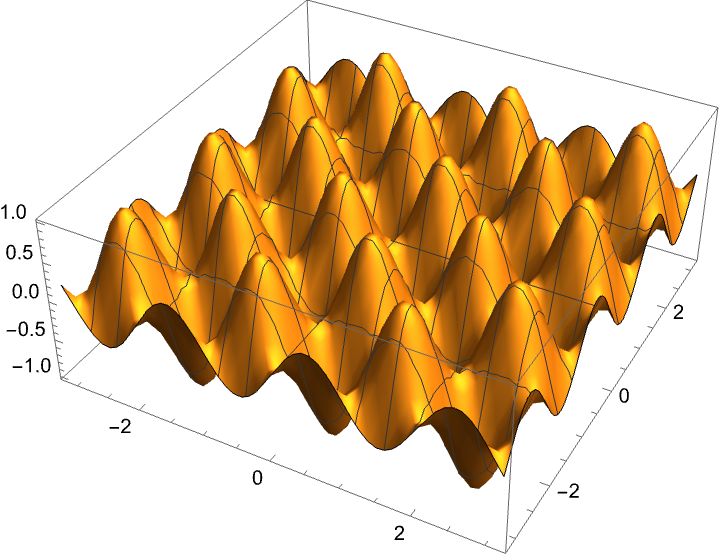
\includegraphics[scale=0.7]{u11.png}
	\end{center}
	Now with $u_{2, 1}(x, y, t) = \sin(\frac{2 \pi x}{L}) \sin(\frac{\pi y}{L})$:
	\begin{center}
		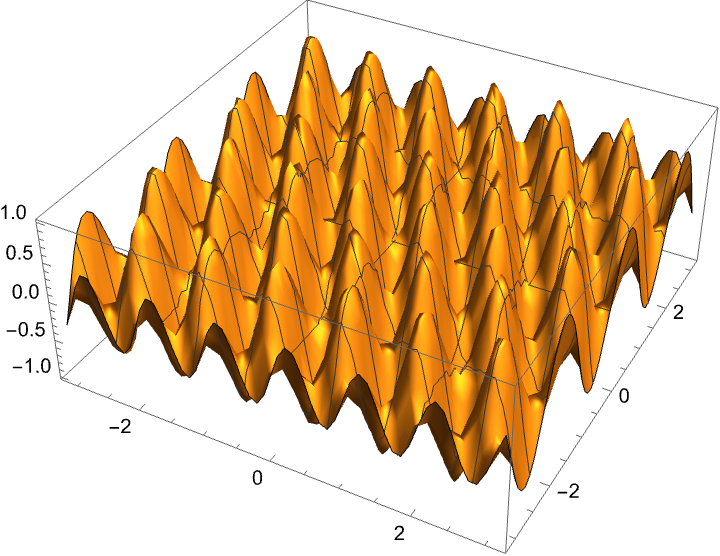
\includegraphics[scale=0.7]{u21.png}
	\end{center}
	Here's $u_{1, 2}(x, y, t) = \sin(\frac{\pi x}{L}) \sin(\frac{2 \pi y}{L})$:
	\begin{center}
		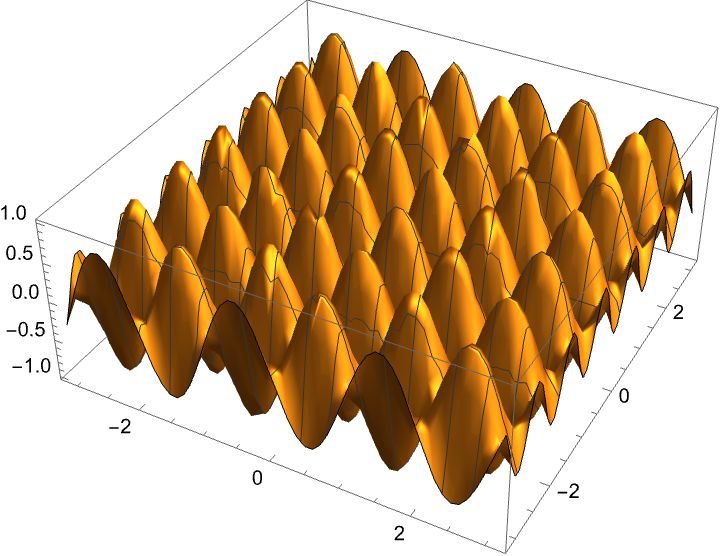
\includegraphics[scale=0.7]{u12.png}
	\end{center}
	And finally, $u_{2, 2}(x, y, t) = \sin(\frac{2 \pi x}{L}) \sin(\frac{2 \pi y}{L})$:
	\begin{center}
		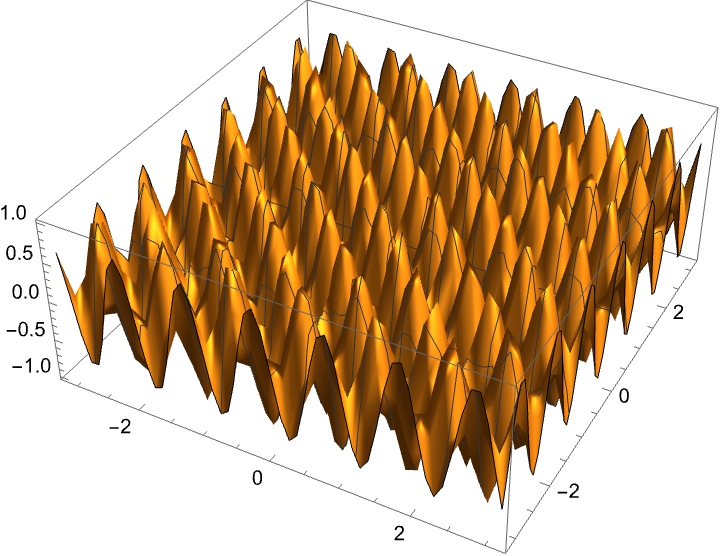
\includegraphics[scale=0.7]{u22.png}
	\end{center}
	Unfortunately, I would animate these but it's impossible to put them into a PDF. Also, Mathematica's
	animation tool isn't the greatest for these kind of plots. 
\end{solution}

\phline
%%%%%%%%%%%%%%%%%%%%%%
\paragraph{}
The general solutions satisfying all of our superposable boundary conditions from (b) is
	\begin{equation*}
		u(x,y,t) = \sum_{n=1}^{\infty}\sum_{m=1}^{\infty} b_{n,m}u_{n,m}(x,y,t).
	\end{equation*}
If we plug in the remaining condition we find
	\begin{equation*}
		u_{0}(x,y) = \sum_{n,m} b_{n,m}\sin(n\pi x/L)\sin(m\pi y/L).
	\end{equation*}
The $b_{n,m}$ can be found via a 2D trigonometric Fourier series,
	\begin{equation*}
		b_{n,m} = \left(\frac{2}{L}\right)^{2}\int_{0}^{L}\int_{0}^{L}\sin(n\pi  x/L)\sin(m\pi y/L)u_{0}(x,y)dxdy.
	\end{equation*}
Suppose we have with initial condition $u_{0}(x,y) = \delta(x-L/2)\delta(y-L/2)$.

\paragraph{(h)}
Find the coefficients $b_{n,m}$ and give a final form for $u(x,y,t)$!
\extrasubpart{Try animating your solution.}

\begin{solution}
	We're given $u_0(x, y) = \delta(x - L / 2) \delta(y - L / 2)$, so we just have to throw this 
	into the formula for $b_{n, m}$:
	\begin{align*}
		b_{n, m} &= \left( \frac{2}{L} \right)^2 \int_0^L \int_0^L \sin\left(\frac{n \pi x}{L} \right) 
		\sin(\frac{m \pi y}{L}) \delta\left(x - \frac{L}{2}\right) \delta\left(y - \frac{L}{2}\right) dx dy\\
				 &= \left( \frac{2}{L} \right)^2 
				 \left[\int_0^L \sin(\frac{n \pi x}{L})\delta\left(x - \frac{L}{2}\right) dx\right] 
				 \left[\int_0^L \sin(\frac{m \pi y}{L}) \delta\left( y - \frac{L}{2} \right) dy\right] 
	\end{align*}
	And now we use the property of the Dirac delta:
	\[
	\int_a^b f(x) \delta(x - x_0) = \begin{cases}
		f(x_0) & a < x_0 < b\\ 
		0 & \text{else}
	\end{cases}
	\] 
	So since $0 < \frac{L}{2} < L$, then this expression for $b_{n, m}$ evaluates to:
	\begin{align*}
		b_{n, m} &= \left( \frac{2}{L} \right)^2 \sin( \frac{n \pi L / 2}{L}) \sin(\frac{m \pi L / 2}{L})\\
				 &= \left(\frac{2}{L}\right)^2 \sin(\frac{n \pi}{2}) \sin(\frac{m \pi}{2})
	\end{align*} 
	Therefore, putting it all together, the final form for $u(x, y, t)$ is:
	\[
		u(x, y, t) = \left( \frac{2}{L} \right)^2\sum_{n = 1}^\infty \sum_{m = 1}^\infty \sin(\frac{n \pi}{2})
		\sin(\frac{m \pi}{2}) \sin(\frac{n \pi x}{L}) \sin(\frac{m \pi y}{L}) \cos(\left(\sqrt{n^2 + m^2}\right) \frac{\pi vt}{L})
	\] 
	I do have to say that writing that down was very satisfying, both because it's a nice result but also because
	it's the last problem in this course!
\end{solution}
\bigskip
\dphline
\pagebreak
%%%%%%%%%%%%%%%%%%%%%%%%%%%%%%%%%%%%%%%%%%%%%%%%%%%%%%%%%%%%%%%%%%%%%%%%%%%%%%%%
\section*{Problem 10.3 - Temperature Distribution in a Sphere (Not for Credit)}
\relevid{Solving PDEs with Separation of Variables;
Separation of Variables and Boundary Value Problems;
Example - A Steady State Temperature Distribution}

\paragraph{}
Consider a sphere of radius $R$.  We wish to find the steady state temperature in the sphere $T(r,\theta,\varphi)$ given boundary conditions at the surface of the
sphere $r=R$.
The temperature distribution in the steady state is given by a Laplace equation,
	\begin{equation*}
		\nabla^{2}T(r,\theta,\varphi) = 0.
	\end{equation*}
Recall that the Laplacian in spherical coordinates is given by
	\begin{equation*}
		\nabla^{2}f(r,\theta,\varphi) = \frac{1}{r^{2}}\pdiff{}{r}\left(r^{2}\pdiff{f}{r}\right) + \frac{1}{r^{2}\sin\theta}\pdiff{}{\theta}\left(\sin\theta\pdiff{f}{\theta}\right) 
			+ \frac{1}{r^{2}\sin^{2}\theta}\ppdiff{f}{\varphi}.
	\end{equation*}


%%%%%%%%%%%%%%%%%%%%%
\paragraph{(a)}		\extrapart
Perform a separation of variables in spherical coordinates, $T(\vec{x}) = R(r)Y(\theta,\varphi)$, to separate out the radial and angular independent variables in the
Laplace equation. You should
wind up with an ODE for $R(r)$ and a PDE for $Y(\theta,\varphi)$.  
\spoilers{Remember, you want to manipulate the equation so that each term only depends on a particular subset of the independent variables.  Here, we want terms that only
depend on $r$ and terms that only depend on the angles.}

\begin{solution}
	Plugging it all into our differential equation, we have:
	\[
		\nabla^2 T(\vec x) = \frac{1}{r^2}\pdv{r}\left( r^2 \pdv{R}{r} \right) Y(\theta, \phi) 
		+ \frac{R}{r^2 \sin \theta }\pdv{\theta}\left( \sin \theta \pdv{Y}{\theta} \right) 
		+ \frac{R}{r^2 \sin^2 \theta}\pdv[2]{Y}{\phi} = 0
	\] 
	Then, we can divide through by $\frac{YR}{r^2}$ (or equivalently, multiply by $\frac{r^2}{YR}$:
	\begin{align*}
		\frac{1}{r}\pdv{r}\left( r^2 \pdv{R}{r} \right) 
		+ \frac{1}{Y \sin \theta}\pdv{\theta}\left( \sin \theta \pdv{Y}{\theta} \right) 
		+ \frac{1}{Y \sin^2 \theta }\pdv[2]{Y}{\phi} = 0
	\end{align*}
	The first term is a pure function of $r$, while the remaining two terms depend on $\phi, \theta$. 
	Therefore, if we separate these (with the algebraic relation $c_r + c_\theta = 0$, we get:
	\begin{align*}
		c_r &= \frac{1}{R}\pdv{r}\left( r^2 \pdv{R}{r} \right)  \\
			&= \frac{1}{R}\left[r^2 \pdv[2]{R}{r} + 2r \pdv{R}{r}\right] \\
			&= \frac{r^2}{R}\pdv[2]{R}{r} + \frac{2r}{R}\pdv{R}{r} 
	\end{align*}
	Multiplying both sides by $R$ and then moving the constant over, we get:
	\[
		r^2 \pdv[2]{R}{r} + 2r \pdv{R}{r} - c_r R = 0
	\] 
	As for the angular equation, we separate out the other part:
	\begin{align*}
		c_\theta &= \frac{1}{Y\sin \theta}\pdv{\theta}\left( \sin \theta \pdv{Y}{\theta} \right) 
		+ \frac{1}{Y \sin^2 \theta} \pdv[2]{Y}{\phi}
	\end{align*}
	Multiplying both sides by $Y$ and then moving the constant over:
	\[
		\frac{1}{\sin \theta}\pdv{\theta}\left( \sin \theta \pdv{Y}{\theta} \right) 
		+ \frac{1}{\sin^2 \theta} \pdv[2]{Y}{\phi} - c_\theta Y = 0
	\] 
\end{solution}

\phline
%%%%%%%%%%%%%%%%%%%%%
\paragraph{}
Let the separation coefficient for the radial ODE be $\ell(\ell+1)$, where $\ell$ is a non-negative integer.  (This weird form of the separation constant is 
due to a quantization condition when solving the angular equation).  The radial equation should then be
	\begin{equation*}
		r^{2}\frac{d^{2}R}{dr^{2}} + 2r\frac{dR}{dr} - \ell(\ell+1)R = 0.
	\end{equation*}
This is a Euler-Cauchy-type problem!

%%%%%%%%%%%%%%%%%%%%%
\paragraph{(b)}		\extrapart
Solve using whatever method you would like to find the two linearly independent solutions to this equation!  You can use physical considerations (the temperature doesn't 
diverge to infinity anywhere in the sphere!) to eliminate one of the two solutions.

\begin{solution}
	After some digging through Wikipedia, I found that an ansatz of the form $R(r) = r^m$ works 
	for this type of differential equation. Computing derivatives:
	\begin{align*}
		R'(r) &= mr^{m-1}\\
		R''(r) &= m(m-1)r^{m-2}
	\end{align*} 
	Therefore, plugging this into our differential equation:
	\[
		r^2 m(m-1) r^{m-2} + 2r m r^{m-1} - \ell(\ell+1) = 0
	\] 
	We find that each term has an $r^m$, so we can divide that out. Therefore, we're left with the 
	equation:
	\[
	m^2 + m - \ell(\ell+1) = 0
	\] 
	Using the quadratic formula to solve for $m$, we get:
	\[
		m_{\pm} = \frac{-1 \pm \sqrt{1 + 4\ell(\ell+1)}}{2} 
	\] 
	Since $\ell$ is a non-negative number, we find that $m_+$ is positive, while $m_-$ is negative. In 
	order for our equation to make sense, we don't want any infinities in our solution. This means that the
	negative solution must 
	be inadmissible, since a negative exponent will have a discontinuity at $r = 0$, where the 
	solution diverges to infinity. Therefore, we can only admit the positive solution.
\end{solution}
\phline
%%%%%%%%%%%%%%%%%%%%%
\paragraph{}
The PDE you got from part (a) defines the \heavydef{spherical harmonics} $Y_{\ell}^{m}(\theta,\varphi)$,
	\begin{equation*}
		\frac{1}{\sin\theta}\pdiff{}{\theta}\left(\sin\theta\pdiff{Y}{\theta}\right) 
			+ \frac{1}{\sin^{2}\theta}\ppdiff{Y}{\varphi} = -\ell(\ell+1)Y(\theta,\varphi),
	\end{equation*}
where the index $m$ is introduced in a second separation of variables into a polar and azimuthal part $Y(\theta,\varphi) = \Theta(\theta)\Phi(\varphi)$.  In particular,
	\begin{equation*}
		\frac{d^{2}\Phi}{d\varphi^{2}} = -m^{2}\Phi(\varphi).
	\end{equation*}

\paragraph{(c)}		\extrapart
Show that in order for our azimuthal part to be periodic ($\Phi(\varphi+2\pi)=\Phi(\varphi)$) we must have $m\in\mathbb{Z}$.
Show that the functions $\{x/r, y/r, z/r\}$ all solve the spherical harmonic equation given above for a certain value of $\ell$.  What is $\ell$ for these functions?

\begin{solution}
	The differential equation in question has oscillatory solutions of the form $e^{ikx}$. Specifically, 
	the general solution is a linear combination of these:
	\[
		\Phi(\phi) = Ae^{im \phi} + Be^{- im \phi}
	\] 
	In order to enforce the periodic condition, we have:
	\[
		\Phi(\phi + 2\pi) = Ae^{im (\phi + 2\pi)} + Be^{-im(\phi + 2\pi)} = Ae^{im \phi} e^{im(2\pi)} 
		+ Be^{-im \phi} e^{-im 2\pi}
	\] 
	the only way for this to equal $\Phi(\phi)$ is if $e^{2\pi i m} = e^{- 2\pi i m} = 1$, and this condition 
	requires that $m$ is an integer. As for the functions $\{x / r, y / r, z /r\}$, let's start with 
	$\frac{x}{r} = \sin \theta \cos \phi$:
	\[
		\frac{1}{\sin \theta}\pdv{\theta}\left( \sin \theta \cos \theta \cos \phi \right) 
		+ \frac{1}{\sin^2 \theta} \sin \theta (-\cos \phi) = -\ell(\ell+1)\sin \theta \cos \phi 
	\]
	After some algebra, we get:
	\[
	\cos^2 \theta - \sin^2 \theta - 1 = -\ell(\ell+1)\sin^2 \theta \implies -2 \sin^2 \theta = -\ell(\ell+1)
	\sin^2 \theta 
	\] 
	So we find that for $\frac{x}{r}$, we get $\ell= 1$. Now for $\frac{y}{r} = \sin \theta \sin \phi$:
	\[
		\frac{1}{\sin \theta}\pdv{\theta}(\sin \theta \cos \theta \sin \phi) 
		+ \frac{1}{\sin^2 \theta}\sin \theta (- \sin \phi) = -\ell(\ell+1) \sin \theta \sin \phi
	\] 
	Again, simplifying this algebra, we actually get the same equation as earlier with $\frac{x}{r}$:
	\[
	\cos^2 - \sin^2 - 1 = -\ell(\ell+1) \sin^2 \theta \implies \ell = 1
	\] 
	Finally, for $\frac{z}{r} = \cos \theta$:
	\[
		\frac{1}{\sin \theta}\pdv{\theta}(-\sin^2 \theta) = -\ell(\ell+1) \cos \theta
	\] 
	Simplifying, we get:
	\[
	-2 \cos \theta = -\ell(\ell+1) \cos \theta 
	\] 
	So we also get $\ell = 1$. 
\end{solution}


\endofhomework
\addfooter
%%%%%%%%%%%%%%%%%%%%%%%%%%%%%%%%%%%%%%%%%%%%%%%%%%%%%%%%%%%%%%%%%%%%%%%%%%%%%%%%
\end{document}

